%%%%%

\documentclass[review,3p,times,12pt,number]{elsarticle}
\usepackage{amsmath}
\usepackage{amssymb}
\usepackage{multicol,multirow,amsthm,subfigure,textcomp}
\usepackage{booktabs}

\begin{document}

\begin{frontmatter}

\journal{International Journal of Information Technology \& Decision Making}
\title{Textual Sentiment of Chinese microblog toward the Stock Market}
%\author[shu]{Ning Wang \corref{cor}}
%\ead{ningwang@shu.edu.cn}
%
%\author[qtg]{Yibo Chen}
%\ead{chenyibo1029@gmail.com}
%
%\author[ustc]{Tao Yan}
%\ead{yantao86@mail.ustc.edu.cn}
%
%\author[nus]{Andrew Lim}
%\ead{alim.china@gmail.com}
%\cortext[cor]{Corresponding author.}
%
%\address[shu]{Department of Information Management, School of Management, Shanghai University, Shanghai, China}
%\address[qtg]{Shanghai Liangyou Asset Management Company Limited, Shanghai, China}
%\address[ustc]{Department of Management Science, School of Management, University of Science and Technology of China, China}
%\address[nus]{Department of Industrial \& Systems Engineering, National University of Singapore, Singapore}

\begin{abstract}
In this paper, text mining and statistical models are deployed to explore the relationship between the Shanghai Stock Exchange Composite
Index and the collective emotions of individual investors.
The emotions of individual investors are quantified by extracting and aggregating investor online posts that contain finance-related keywords.
To identify a set of finance-related keywords, three years of blogs from a famous financial blog site are segmented by an automatic text segmentation method; meanwhile, in the literature of social media, people typically select keywords manually.
Posts that discuss the keywords are extracted out of all types of topics from Sina Weibo, the largest microblog platform in China. Statistical results reveal the relationship between daily posts and daily opening prices with a one-day lag, which indicates the existence of information (news) propagation lag. This study contributes to the existing literature by demonstrating that the microblog sentiment level reports can be quantitatively incorporated as a proxy to provide valuable support to portfolio decision making.
\end{abstract}

\begin{keyword}
microblog \sep Chinese stock market \sep textual sentiment \sep emotions of investors
\end{keyword}

\end{frontmatter}


\section{Introduction}
China has become one of the fastest-growing major economies in the world. The daily average turnover of the Shanghai Stock Exchange (SSE) ranks seventh in the world. Examining its market movements is of considerable importance. As an emerging market, the SSE consists of individual investors as major players. Psychological research has indicated that emotions, in addition to information, have a significant role in human decision making \cite{Dolan2002}. The investment decisions of individual investors are more likely to be influenced by their emotions. A reasonable assumption is that when many individual investors hold bullish views, their joint investment decisions are more likely to generate an upward momentum on the stock market. Similarly, more bearish views may generate a downward momentum. Such momentum, together with other factors (i.e., economic conditions, performance of listed companies, and investment decisions of institutional investors), jointly determine stock prices. A positive correlation may exist between the number of bullish (bearish) views and the upward (downward) movement of stock markets.\\
\indent
Social media provides a valuable source for mining public views due to their distinctive features. First, a huge number of active users post their views or share their activities. Second, users who are linked up with each other in online social media are usually friends in reality or people who share similar interests. Thus, such posts typically reflect the true viewpoints of users. Third, posts are timely (i.e., they reflect the recent activities or opinions of users). In terms of successful social media, Facebook and Twitter are the most typical examples. In the Chinese environment, the counterpart of Twitter is Sina Weibo, one of the largest forms of social media in China; it was launched in August 2009. As of September 2016, Sina Weibo has 297 million monthly active users and 100 million posts each day. This paper uses data from Sina Weibo to conduct analysis.\\
\indent
Collected posts are natural language, which must be processed by text mining tools before they can be understood and used by computers. Text mining, also known as text analysis, is the process of deriving knowledge for automated processing from primary text, which normally undergoes structuring (i.e., parsing, adding linguistic features, and removing auxiliary components). Typical text mining tasks include text categorization, text clustering, concept/entity extraction, production of granular taxonomies, sentiment analysis, document summarization, and entity relation modeling (i.e., learning relations between named entities). Text mining involves a number of techniques, such as lexical analysis to study word frequency distributions, pattern recognition, tagging/annotation, information extraction, data mining techniques, including link and association analysis, visualization, and predictive analytics. The objective is to transform text into data for further analysis by applying natural language processing and analytical methods. Aside from the earliest application areas such as life sciences research and government intelligence, text mining has increasing applications in business, such as simple queries and analysis of fielded numerical data.\\
\indent
This paper verifies the rationality of the market from the perspective of behavioral finance. Text mining tools and statistical modeling are employed to investigate the relationship of the Shanghai Stock Exchange Composite Index (SSECI) movements with the viewpoints of individual investors. Viewpoints are quantified by analyzing and aggregating the online posts of individual investors that are related to stock markets, in which the major challenge lies in how to automatically identify a set of suitable keywords. Statistical results of posts from Sina Weibo suggest a relationship between collective viewpoints reflected on Sina Weibo and movements of the SSECI. This study contributes to the existing literature by demonstrating that the microblog sentiment level reports can be quantitatively incorporated as a proxy to provide valuable support to portfolio decision making.

\section{Recent work}
\label{sec:weibo:lr}
As a response to the complications faced by traditional finance theories, behavioral finance has emerged as a new approach in financial markets. In general, behavioral finance argues that some financial phenomena can be better apprehended under the assumption that some players are not fully rational. More definitely, it investigates what happens when tenets that underlied individual rationality are relaxed \cite{Barberis2002}. Behavioral finance has provided proofs that financial decisions are significantly driven by emotions and moods \cite{Nofsinger2005}. Recent study in behavioral economics shows that stock markets are driven by ``fear and greed". %Broadly speaking, two types of sentiment have been studied \cite{Kearney2014}. The first type is investor sentiment -- beliefs about future cash flows and investment risks that are not justified by the facts at hand \cite{Baker2007}. The second type of sentiment is text-based or textual sentiment -- the degree of positivity or negativity in financial texts.\\
\indent
%A substantial body of investor sentiment literature focuses on measuring investor sentiment using various approaches, as well as determining its effect on individual stocks and the overall market.

We have divided the related literature into four categories according to research emphasis shown in their articles: various approaches to measure investor sentiment, stock comovement or movement, stock market indices and the relationship between investors sentiment and market variables.

\subsection{Various approaches to measure investor sentiment}
%Liu et al.~\cite{liu2006predicting} studied the influence of community sentiment on the stock market where the community sentiment is deduced from the posts on the finance forum of Yahoo Finance using the expert classification method. They also proposed a trading strategy that one should buy stocks when the market sentiment is low and sell stocks when the market sentiment is high.
Schumaker and Chen~\cite{schumaker2009textual} analyzed financial news articles through a predictive machine learning approach and investigated their effect on stock quotes covering the S\&P 500 stocks. They revealed that subjectivity in financial news articles influences the market trading immediately after the release of news. Adding article terms into prediction models exhibits the best performance in getting close to the actual stock price.
A novel approach combining text mining, feature selection and a decision tree model was proposed in Nasseri et al.~\cite{Nasseri2015Quantifying} to quantify and predict investor sentiment from a stock microblogging forum (StockTwits) of Dow Jones Industrial Average companies. They constructed a trading strategy based on a predetermined investment hypothesis and it achieved a promising performance and outperformed random investment strategies. Their findings did confirm that StockTwits postings contain valuable information and lead trading activities in capital markets.
Machine learning was also employed to conduct sentiment classification of data in order to estimate future stock prices in Romanowski and Skuza~\cite{Romanowski2017}.
Oliveira el al.~\cite{Oliveira2017The} proposed a robust method to confirm the usefulness of microblogging data to forecast stock market variables: returns, volatility and trading volume of diverse indices and portfolios.
Dash and Maitra~\cite{Dash2017Does} investigated the relationship using a broad set of implicit sentiment proxies and value-weighted market indices. They used the wavelet method to decompose sentiment variables and stock returns into different timescale frequencies and found a strong effect of sentiment on return both in the short-and long-run. The study lent support to the fact that investments activities can not be delinked from sentiment whether investors were short-term or long-term traders. Another research about revisiting the investor sentiment-stock returns relationship with the wavelet method can be seen in Lao et al.~\cite{Lao2018Revisiting}.
In addition, the wavelet method was applied to study the relationship of investor sentiment on stock market volatility in Maitra and Dash~\cite{Maitra2017Sentiment}.

\subsection{Stock comovement or movement}
%Sentiment analysis and machine learning principles are applied to study causation between public collective sentiment and market movements in Rao and Sirvastava~\cite{Rao2012TweetSmart}.
%Chen and Lazer~\cite{Chen2013Sentiment} constructed a model to investigate the relationship between Twitter feed content and stock market movement and put it to the test on real market data using a mock portfolio. The result indicated that the model was successful in generating additional profit.
Smailovic et al.~\cite{Smailovi2013Predictive} showed that sentiment polarity (positive and negative sentiment) can indicate stock price movements a few days in advance by using the Granger causality test.
Liu et al.~\cite{Liu2015A} studied the stock return comovement through a social-media-based approach and they proposed a novel clustering model to both identify homogeneous stock groups and predict stock comovement with respect to firm-specific social media metrics. The results showed that with simple metrics, social media data can produce better results compared to industry categories.
Li et al.~\cite{Li2017Discovering} studied how public sentiment, as reflected on social media, can be used to predict stock price movement of a particular publicly-listed company. They proposed the technique called Social Media Data Analyzer-Sentiment Analysis (SMeDA-SA) to mine Twitter data for sentiment analysis and then predict the stock movement of specific listed companies. The result indicated that the stock movement of many companies can be predicted rather accurately with an average accuracy over 70\% with SMeDA-SA.



\subsection{Stock market indices}
Gilbert and Karahalios~\cite{Gilbert2010} estimated the anxieties, worries and fears from a data set of more than over 20 million posts on the site LiveJournal. Using a Granger-causal framework, Gilbert and Karahalios argued that increases in the expressions of anxiety, evidenced by computationally-identified linguistic features, predict the downward pressure on the S\&P 500 index.
Bollen et al.~\cite{bollen2011twitter} investigated whether the measurements of collective mood states derived from large-scale Twitter feeds are correlated to the value of the Dow Jones Industrial Average over time. They analyzed the text content of daily Twitter feeds using two mood tracking tools, namely OpinionFinder that measures positive versus negative mood and Google-Profile of Mood States (GPOMS) that measures mood in terms of six dimensions (i.e., Calm, Alert, Sure, Vital, Kind, and Happy).
Similarly, Zhang et al.~\cite{zhang2011predicting} collected six months of Twitter posts and analyzed the emotions reflected in the posts. They indicated that the emotions can be used to predict the Dow Jones, NASDAQ and S\&P 500 indices.
Sun et al.~\cite{Sun2016Trade} proposed the sparse matrix factorization (SMF) model and the model outperformed most baseline models after testing this model on data spanning from 2011 to 2015 on a majority of stocks listed in the S\&P 500 Index. They also concluded that increasing the frequency of predictions does not seem to improve prediction accuracy.
Gao and Yang~\cite{Gao2017Forecasting} constructed stock index futures sentiment and stock index sentiment at daily, weekly, and monthly frequencies and tested the predictive power of mixed-frequency stock index futures sentiment and mixed frequency stock index futures sentiment on stock index futures returns at different frequencies by using the Mixed-Data Sampling (MIDAS) model. The empirical results confirmed that mixed-frequency stock index futures sentiment and mixed-frequency stock index sentiment were systemic and important factors in futures price.


\subsection{The relationship between investors sentiment and market variables}
%Barberis and Huang~\cite{Barberis2008} revealed that the utility of these investors with the cognitive biases of loss aversion, mental accounting, and probability weighting improves if they hold securities with positively skewed returns. Consequently, these investors demand lower risk compensation for positively skewed stocks, thus weakening the risk-return tradeoff.
Barber and Odean~\cite{Barber2008}, Sprenger and Welpe~\cite{Sprenger2014Tweets} mainly analysed the relationship between investors sentiment and stock returns and trading volumes, while the influence of investors sentiment on stock price was investigated in Chen~\cite{schumaker2009textual}, Nguyen el al.~\cite{Nguyen2015Sentiment} and Schumaker and Guo et al.~\cite{Guo2017Can}.
Debata et al.~\cite{Debata2017Investor} examined the impact of local and foreign investor sentiment on emerging stock market liquidity. They found a positive effect of investor sentiment on liquidity. It also revealed that foreign investor sentiment significantly influenced emerging stock market liquidity in their results. Other research about the investor sentiment on stock market liquidity can be seen in Baker and Stein~\cite{baker2004market} and Liu~\cite{Liu2015Investor}.

There are many articles intensively studying the effect of investors sentiment on stock return, volatility and trading volumes.
For example, Uygur and Tas~\cite{Uygur2014} adopted an international approach using the weekly market index returns of the United States, Japan, Hong Kong, United Kingdom, France, Germany, and Turkey. The weekly trading volumes of these indexes are regressed against a group of macroeconomic variables and the residuals are used as proxies for investor sentiment. Significant evidence confirmed that the asymmetric volatility in these market indexes and earning shocks have more influence on conditional volatility when the sentiment is high.
You can also read the related literature about this research in Oliveira et al.~\cite{Oliveira2013On}, Checkley et al.~\cite{Checkley2017The} and Oliveira el al.~\cite{Oliveira2017The}.

Most studies put their emphasis on the relationship between investors sentiment and stock returns.
Baker and Wurgler~\cite{baker2006} used simple theoretical arguments, historical accounts of speculative episodes, and a set of novel empirical results to demonstrate that investor sentiment induces significant cross-sectional effects. The cross-section of future stock returns is conditional on beginning-of-period proxies for sentiment; several firm characteristics that display no unconditional predictive power actually hide strong conditional patterns that become visible only after conditioning on sentiment.
Yu and Yuan~\cite{Yu2011} demonstrated the influence of investor sentiment on the mean-variance tradeoff of the market. The expected excess returns of the stock market are positively related to the conditional variance of the market in low-sentiment periods but unrelated to variance in high-sentiment periods. Yu and Yuan also reported that the negative correlation between returns and contemporaneous volatility innovations is considerably stronger in the low-sentiment periods.
Pineiro et al.~\cite{Pi2016Examining} analyzed the links between different combinations of causal conditions (market variables and variables related to social media activity) in contrast to analyze if the microblog sentiment can predict stock returns.
You et al.~\cite{You2017Twitter} observed that the causal relationship from happiness sentiment to stock returns existed only in high quantiles interval. The causal relationship from stock returns to happiness sentiment existed only in the tail area.
Xu and Zhou~\cite{Xu2018A} investigated how short-term investor sentiments predict cross-sectional stock returns and constructed a weekly-frequency aligned sentiment index using the partial least squares approach. They confirmed that sentiment changes have positive impacts on future portfolio returns and found that the aligned sentiment indexes have strong return predictability  for small-size portfolios.
Ruan et al.~\cite{Ruan2018Cross} employed multifractal detrended cross-correlation analysis (MF-DCCA) to investigate the cross-correlation between individual investor sentiment and Chinese stock market return.

%Studies on textual sentiment aim to deploying sentiment analysis techniques to collect the sentiment behind information sources, such as Google query and microblogging posts, to facilitate the identification of the relationship between market moods and market movements. The term ``tone'' (positive or negative) is used to refer to the sentiment.

%In terms of the application of social media to other markets, social media have been utilized to predict spikes in book sales \cite{gruhl2005predictive}. Mishne and Glance and Allen and Karjalainen~\cite{Mishne2006,Asur2010} used blogger sentiments and chatters from Twitter.com to forecast box-office revenues for movies. Liu et al.~\cite{Liu07arsa} studied the problem of mining sentiment information from blogs and investigated the means of using such information for predicting product sales performance. O'Connor et al.~\cite{Oconnor2010} analyzed several surveys on consumer confidence and political opinions from 2008 to 2009, and revealed that consumer confidence and political opinions correlate to the frequencies of sentiment words in contemporaneous Twitter messages. de Vries et al.~\cite{deVries2012} investigated the determinants of brand post popularity on brand fan pages. To predict NFL game outcomes, Schumaker et al.~\cite{Schumaker2017} examined the application of technical stock market techniques to sentiment gathered from social media.\\
\indent
Although the textual sentiment in finance has been studied in the research community, the investigation of the Chinese market using posts in Chinese is lacking. Technically, the Chinese language is highly different from the English language in terms of recognizing words. Moreover, given that microblogging includes miscellaneous information, the process of determining whether a word describes the financial market, rather than other things, is a challenge. This study devises a novel method based on a statistical model to extract finance-related Chinese words from general microblogging posts, and the extracted keywords include both emotional and neutral words.


\section{System Framework}
\label{sec:weibo:sf}
The overall ideology can be briefly summarized as follows. First, a set of $k$ keywords that are relevant to the stock market is determined semi-automatically. Each day, a vector consisting of $k$ variables records the number of daily posts on Sina Weibo, with one variable corresponding to one keyword. The vector to some extent summarizes the collective viewpoints of individual investors on that day. Such vectors are collected for a certain period. Consequently, variables across the observation time can be regarded as time series, thus; yielding a total of $k$ time series. A suitable statistical model is developed to relate SSECI to the $k$ time series. %Statistical analyses are used to isolate those keywords that have significant impact on the index.

\section{Data Collection}
\label{sec:weibo:dp}
Three sources of data are used in this study. The first two sources are Sina financial blogs and Sina Weibo. Sina financial blogs are crawled by computers and stored in a MySQL database. Considering the large volume of Sina Weibo and the limitation of Sina Weibo Company, no Sina Weibo post is downloaded to local computers; instead, the query function of Sina Weibo is used in retrieving the required posts and the demographic information. The third source of data is the SSECI. Daily open prices of the SSECI in the same observation period as Weibo posts are downloaded from a publicly available financial website.\footnote{http://www.gw.com.cn/}. Since posts on Sina Weibo are generally Chinese we have to segment Chinese texts first.

\subsection{Chinese Text Segmentation}
\label{sec:weibo:algo}
Chinese is relatively different from English; delimiting a string of Chinese characters into words is considerably more challenging because no explicit word boundary markers exist, such as the word spaces of written English. A specialized procedure for breaking Chinese sentences into words should be developed. The proposed procedure is based on two concepts, namely, stickiness and entropy.

Stickiness measures the stickiness of characters in words. Characters within a word tend to stick together more often than by chance. Given two characters $C_1$ and $C_2$, they appear together in a text either by chance or as one part of a common word. $f$, $f_1$ and $f_2$ denote the frequencies of $C_1C_2$, $C_1$ and $C_2$ in the text, respectively. If $C_1$ and $C_2$ are independent, then $f\approx f_1 \times f_2$. By contrast, if $f \gg f_1 \times f_2$, then the independent assumption may be reasonably rejected and that $C_1C_2$ is therefore a part of a common word. More broadly, for a token $T$ with $n$ characters, $n-1$ ways of separation that separates $T$ into two substrings $S_1$ and $S_2$ exist. If $T$ is a word, then $S_1$ and $S_2$ resulting from any separation should satisfy $f\gg f_1\times f_2$, where $f$, $f_1$ and $f_2$ denote the frequencies of $T$, $S_1$ and $S_2$ in the text, respectively.
The stickiness of a token $T$ is generally defined as
\begin{equation}
s(T)=\min_{S_1,S_2} \frac{f}{f_1\times f_2}
\end{equation}


A word as a whole entity typically follows or precedes a richer set of characters than a part of it does.
Given a word $W$ and its substring $S$, the stickiness of $S$ is larger than that of $W$. Therefore, if only stickiness is used, then all of the substrings of a word will be detected as words. Although some substrings are indeed words, most substrings do not have any proper meanings and are not qualified as words.

To distinguish words from substrings, information theory is used. If a token $T$ is a substring of $W$, then the expectation is that most occurrences of $T$ in the text should be a part of $W$. Without loss of generality, $C_i$ ($i\in \{1, 2, \ldots, n\}$) denotes a character that immediately precedes $T$ in the text. Suppose $T$ is a suffix of $W$ and the character that immediately precedes $T$ in $W$ is $C_k$, then the occurrences of $T$ and $C_k$ are closely related, and the string $C_kT$ is expected to occur more frequently than any string $C_iT$ ($i\neq k$). By contrast, if $T$ is a word itself, then the occurrences of any string $C_iT$ will be more evenly and the occurrence of $T$ provides more information, namely, it cannot identify the specific letter that precedes $T$ when $T$ appears. Let $n_i$ be the number of occurrences of $C_iT$; thus the entropy of $T$ for prefix is defined as follows:
\begin{equation}
\begin{split}
\label{eqn:entropy}
p_i = n_i / \sum_{j=1}^n n_j \\
e_p(T)= \sum_{i=1}^n[-p_i\log{p_i}]
\end{split}
\end{equation}

A string will be accepted as a word only if its entropy for prefix is sufficiently high. The entropy for suffix can be defined and calculated in a similar manner.

A title is initially delimited into strings by punctuation marks, such as colon, comma, and hyphen. Strings are delimited into words by the following procedure:
\begin{itemize}
    \item {\bf Step 1} For each string, all of the substrings with lengths smaller than $d$ are enumerated, and the obtained substrings are denoted as tokens.
    \item {\bf Step 2}  Tokens with stickiness less than $s$ are removed.
    \item {\bf Step 3} Tokens with entropies for prefix or suffix less than $e$ are removed.
    \item {\bf Step 4} For each token, the occurrences over all of the collected blog titles are counted; tokens with frequency less than $F$ are removed.
\end{itemize}

The parameters $d$, $s$, $e$, and $F$ are determined by experiments.

\subsection{Keyword Selection}
\label{sec:keysel}
A keyword set that contains $k$ finance-related words is determined semi-automatically. The keyword measures the emotions of collective viewpoints; therefore, the set should be as complete as possible so that it captures as much information as possible. As the extant dictionaries and word extraction techniques are not customized to identify finance-specified Chinese words, and different groups of Weibo users tend to develop their own special languages that typically contain shorthand (nonstandard) words, extracting finance-specified Chinese words from Internet is the best choice.\\
\indent
Posts on Sina Weibo to some extant reflect the emotions and viewpoints of investors. Directly using Weibo data is desirable. However, Sina Weibo Company denies the access of computers (i.e., computers cannot automatically download Weibo data). In addition, the data volume is extremely huge to be stored locally even if accessing data is allowed. Thus, the demographic characteristics of the overall Sina Weibo, such as language styles and currently hot topics, cannot be obtained by investigating the entire data space of Sina Weibo.

\indent
To overcome this difficulty, we use the blogs from Sina financial blogs to extract keywords. The reason are that: 1) The language style of blogs and microblogs are similar; 2) Sina lists limited number of financial opinion leaders and these celebrities regularly post commentaries on the stock market. We can download all their posts easily.\\

\subsection{Viewpoint Collection}
We quantify the viewpoints of Sina Weibo users on the stock market as the numbers of keywords that users post.
Sina Weibo Company forbids users from accessing its overall posts, but it provides the public with a search function. The trouble thing is that Sina Weibo company limits the number of acessess in each minute; hence it takes us several months to collect the viewpoints.
For each keyword, the search function is invoked to obtain the numbers of daily posts that contain the specified keyword in the observation period. The time series of each keyword is one variable in the statistical model.



\section{Statistical Modeling}
\label{sec:weibo:model}

The daily opening prices are modeled with the collected viewpoints.

\subsection{Basic Linear Regression Model}
%In mathematical finance, especially the Black-Scholes model, the stock price is often assumed to follow a geometric Brownian motion (GBM); SSECI as a weighted sum of stock prices will also follow a GBM \cite{black1973pricing}.
The short-term movement of a stock is the result of the joint market forces, and the joint market forces can be predicted with certain accuracy based on the viewpoints of a sufficient number of individual investors.The daily opening price of the SSECI on day $d$ is denoted by $o_d$; the linear regression model that links daily returns to the numbers of relevant posts on Sina Weibo is subsequently modeled as follows:

\begin{equation}
	r_d=\frac{ \Delta o_d }{o_{d-1}} = \alpha_0 + \sum_{i=1}^{k} \alpha_i x_{i,d-1} + \varepsilon_d \label{weibo:eqn:predict}
\end{equation}
where $x_{i,d-1}, i=1,2,\cdots, k$ is the number of posts related to the $i$th keyword on day $d-1$. The coefficient $\alpha_i$ represents the relative weight of the $i$th keyword. The actual market dynamics are considerably more complex than the preceding linear model; therefore, an error term $\varepsilon_d$ is introduced to account for those factors that are not captured by this linear model.

The daily return in the index $r_d$ is typically small. For a small number $x, x \approx \ln (1+x)$; therefore, $r_d$ is rewritten as follows:
\[
	r_d=\frac{ \Delta o_d }{o_{d-1}} \approx \ln (1 + \frac{ \Delta o_d }{o_{d-1}}) = \ln (1 + \frac{o_d - o_{d-1}}{o_{d-1}}) = \ln \frac{o_d}{o_{d-1}}
\]

\subsection{Unit Root Testing}
 Several economic time series are unit root processes. Two independent unit root processes may appear highly correlated purely by chance; this phenomenon is called a spurious relationship. A standard technique for minimizing the chance of a spurious relationship is through first difference. The ADF test is applied to each time series $x_i$ to identify the unit root process.

The time series that is not covariance stationary is replaced by its difference. The linear Model \ref{weibo:eqn:predict} is refined as follows:
\begin{equation}
\label{weibo:eqn:unitroot}
\begin{split}
	\ln \frac{o_d}{o_{d-1}} & =   \alpha_0 + \sum_{x_i \in \mathrm I(0)} \alpha_i x_{i,d-1}  + \sum_{x_i \in \mathrm I(1)} \alpha_i \Delta x_{i,d-1}+  \varepsilon_d \\
	\Delta x_{i,d}          & =   x_{i, d} - x_{i, d-1},\quad x_i\in \mathrm I(1)
\end{split}
\end{equation}
where I(0) and I(1) denotes time series that are covariance stationary and not covariance stationary, respectively.

\subsection{Data Normalization and Variable Selection}

To avoid the effect of various magnitudes across different time series $x_i$ and allow a meaningful comparison and interpretation of the result, time series $x_i$ are standardized by computing the $z$-scores:
\begin{equation}
\begin{split}
    z_{i,d}  &  = \frac{x_{i,d} - \overline{x}_i}{\sigma_i}, \quad x_i\in \mathrm I(0)\\
    z_{i,d}  &  = \frac{\Delta x_{i,d}-\overline{\Delta x}_i}{\sigma_i'}, \quad x_i\in \mathrm I(1)
\end{split}
\end{equation}
where $\overline{x}_i$ and $\overline{\Delta x_i}$ are the averages of $x_i$ and $\Delta x_i$ over $d$, respectively. $\sigma_i$ and $\sigma_i'$ are the variances of $x_i$ and $\Delta x_i$ over $d$, respectively.

A stepwise variable selection procedure is subsequently deployed to the linear Model \ref{weibo:eqn:unitroot} to reduce the number of variables. During this step, $\varepsilon_d$ is treated as white noise and the ordinary least square estimation is applied.

\subsection{ARIMA Model for the Error Term}
In Model \ref{weibo:eqn:unitroot}, $\varepsilon_d$ is treated as white noise. Actually, the error term $\varepsilon_d$ includes not only the white noise but also the components that capture the complex dynamics of the index. We model the error term $\varepsilon_d$ by the ARIMA$(p, d, q)$ model:
\begin{eqnarray}
\label{eqn:error}
	\nonumber \varepsilon_d &= \phi(L)^{-1}(1-L)^{-d}\theta(L)\eta_d  \\
	\phi(L)       &= 1-\phi_1 L - \phi_2 L^2 - \cdots - \phi_p L^p \\
	\nonumber \theta(L)     &= 1+\theta_1 L + \theta_2 L^2 + \cdots + \theta_q L^q
\end{eqnarray}
where $L$ denotes the lag operator that operates on an element to produce the previous element, $\phi(L)$ is a polynomial of the degree $p$, $\theta(L)$ is a polynomial of the degree $q$, and $\eta_d$ are independent and identically distributed standard normal random variables.\\
\indent
Deciding the appropriate values for $p$, $d$, and $q$ is crucial in making valid statistical conclusions. A single best means of deciding the appropriate values is lacking; hence, a set of combinations is tested to minimize the risk of selecting the incorrect parameters. Model \ref{eqn:error} is estimated using the Gauss-Newton (G-N) iteration method with each combination of $p$, $d$ and $q$.
A small set of combinations is selected from the combination set based on three commonly used model selection criteria AIC, SC and BIC.\\
\indent
After $p$, $d$, and $q$ are known, Models \ref{weibo:eqn:unitroot} and \ref{eqn:error} subsequently are merged as a model. The coefficients in the merged model are estimated once again using the G-N iteration method.
Moreover, a Granger causality test is performed to test the causality between market returns and the number of Weibo posts.
%The forecasting models for daily high, low and closing prices are developed in the same process as the daily opening price.


\section{Experiments and Analysis}
\label{sec:weibo:ea}

\subsection{Data Collection}
\subsubsection{Demography of blogs}
This subsection discusses the descriptive statistics of the financial blog titles. As the object of interest is Chinese, statistics exclude non-Chinese characters, such as English words and punctuation marks. In the Java program, only chars with Unicode points no smaller than 19,968 and no larger than 171,941 are counted. However, the aforementioned point range includes 154 Chinese punctuation marks, each of which is stored in computers by two Unicode points. To this end, one additional criterion is added to filter out non-Chinese characters; the criterion is that chars with Unicode points in the range [65,072, 65,131] and [65,281, 65,374] are excluded from the Chinese character set.\\
\indent
In the channel of Sina financial blogs, 522 celebrities regularly post commentaries. Up to 328,311 blogs are written by these celebrities. We automatically crawled the titles of posted blogs and stored them in a MYSQL database. An observation of a sample of downloaded titles indicates that the writing style of these titles is similar to that of posts on Sina Weibo. A total of 4,904 Chinese characters exist in the collected set of financial blog titles. Approximately 5,000 Chinese characters are commonly used in Chinese. The number of characters in the collected titles is close to the size of commonly used characters. From the semantic perspective, most of the financial blog titles use oral language; thus, the statistical finding is consistent with the semantic finding.\\
\indent
The statistics in this study indicate that the size of collected titles is 3,799,703 characters. The most frequently appeared character is the one which means ``of", with a frequency of 1.89\%. A total of 636 characters only appear once in titles. Thus, such least used characters have a frequency of only 0.0026\textpertenthousand. The average frequency for all characters is 2.04\textpertenthousand.

\subsubsection{Parameter Tuning of Text Segmentation}
Four parameters $d$, $s$, $e$ and $F$ are involved in text segmentation. According to Table \ref{weibo:tab:wl}\footnote{The table is reproduced from Table 3 of \cite{teahan2000compression}.}, words with five or less characters account for 99.8\% of the overall words. Although this table may over-represent single-character words and underrepresent bigrams, setting $d=5$ is reasonable and appropriate for use.

\begin{table}[htbp]
\caption{Distribution of word length in Chinese corpus}
\label{weibo:tab:wl}
\center
\begin{tabular} {l l l}
\hline
length & words  & characters\\
\hline
1      & 55.6\% & 36.2\%\\
2      & 38.2\% & 49.9\%\\
3      & 4.2\%  & 8.2\%\\
4      & 1.6\%  & 4.0\%\\
5      & 0.2\%  & 0.8\%\\
5+     & 0.2\%  & 0.9\%\\
\hline
\end{tabular}
\end{table}

A corpus of Chinese text is generated to determine other parameters. In the collected Chinese blog titles, all of the tokens with lengths not exceeding five are enumerated, and the frequently appeared 4,000 tokens are selected into the corpus. Each token in the corpus is manually marked as words or non-words. Among the 4,000 tokens, 1,613 tokens are marked as words (set $W_c$) and 2,387 tokens are marked as non-words (set $N_c$). Sequentially,
the proposed algorithm is applied to the text of all of the titles, which yields a set of words (set $W_a$).
Two measurements $p_w$ and $p_n$ are used in measuring the precision to identify words and non-words, respectively.
\begin{eqnarray*}
p_w & = &  \frac{|W_c\cap W_a|}{|W_c|}\\
p_n & = &  \frac{|N_c|-|N_c\cap W_a|}{|N_c|}\\
%p   & = &  \frac{2*p_w*p_n}{p_w+p_n}
\end{eqnarray*}

The testing range of stickiness is [0,100] with an incremental of 0.01, and the testing range of entropy is [0,3] with an incremental of 0.1.
Figure \ref{weibo:fig:sepw} shows the effects of stickiness and entropy on $p_w$. Given that $p_w$ decreases as the stickiness and entropy thresholds increase, the horizontal and depth axes are displayed in a reverse order. Thus, $p_w$ is more sensitive to the entropy than to the stickiness.
\begin{figure}[htbp]
\centering
    \label{weibo:fig:sepw}
    \resizebox{0.7 \textwidth}{!}{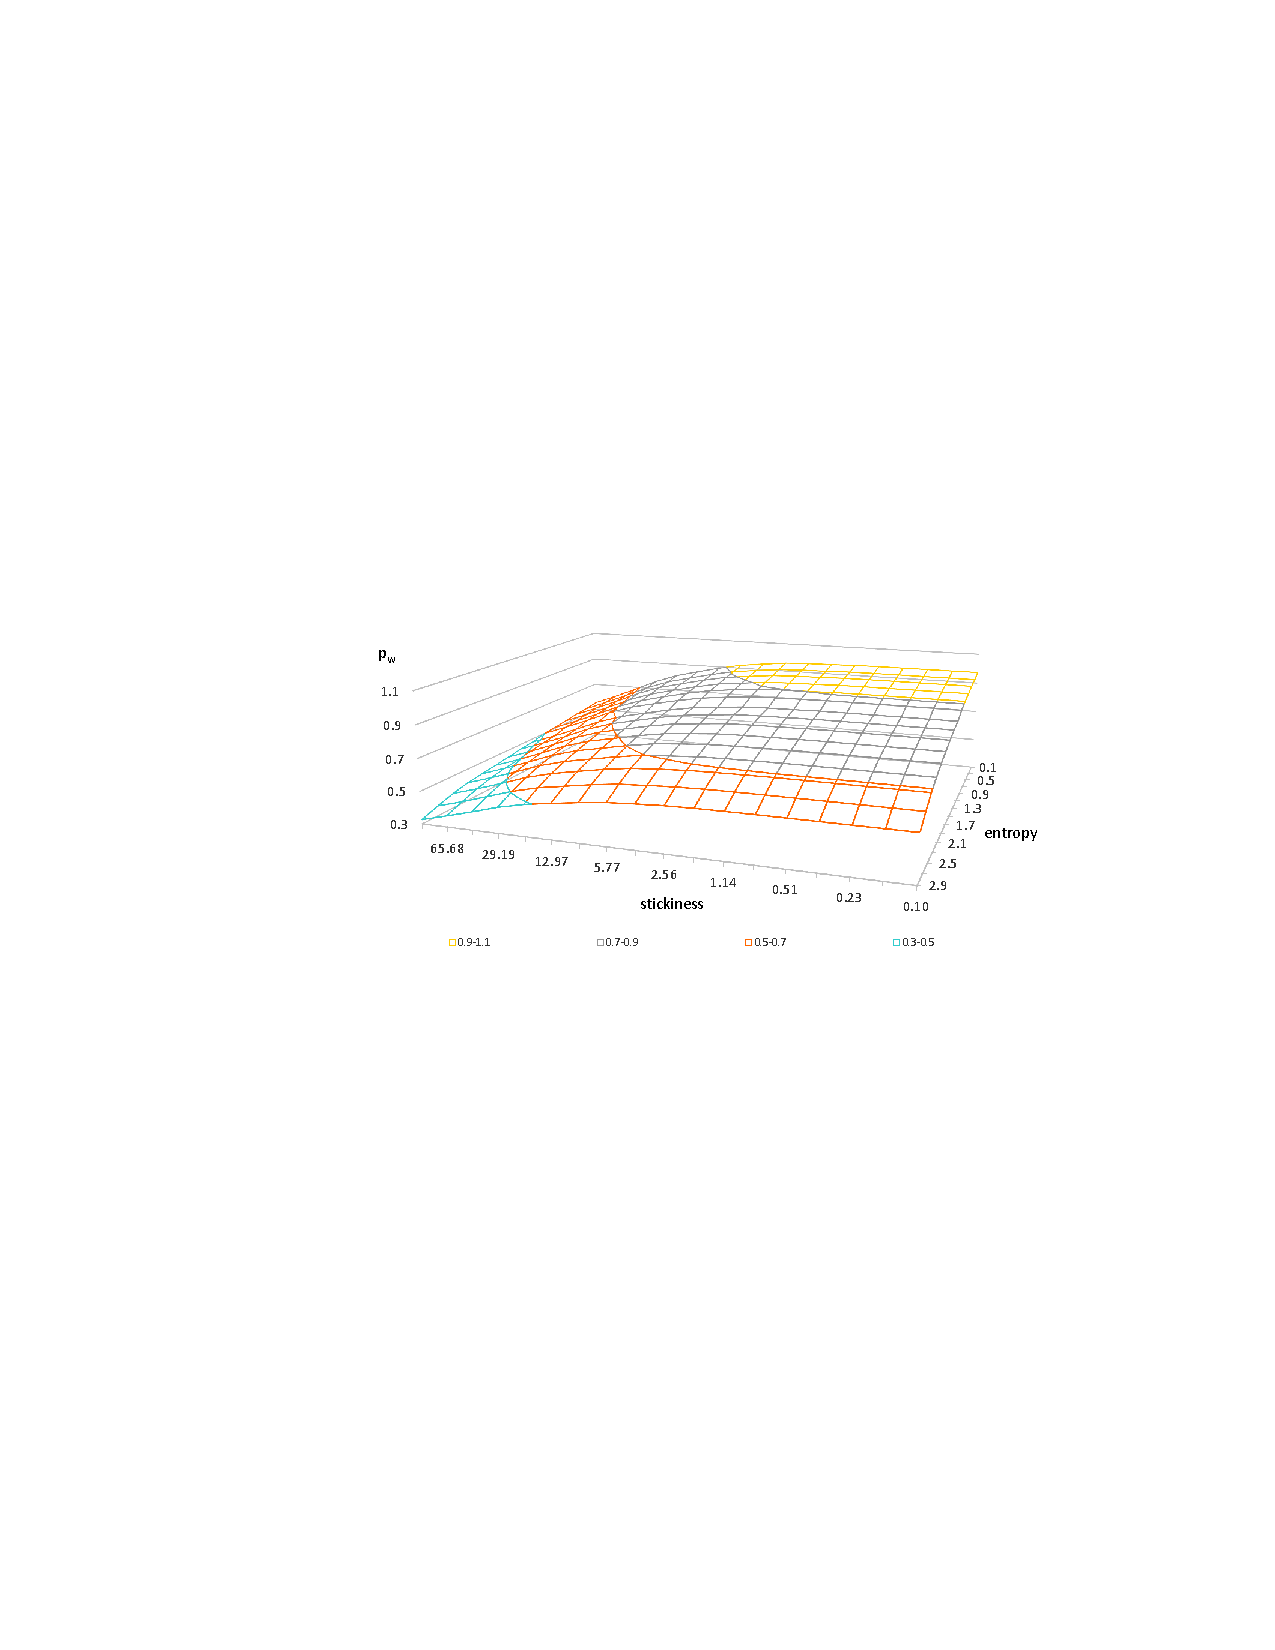
\includegraphics{figure/word_extra_pw.pdf}}
\caption{Effects of stickiness and entropy on $p_w$}
\end{figure}

Figure \ref{weibo:fig:sepn} illustrates the effects of stickiness and entropy on $p_n$. $p_n$ increases as stickiness and entropy thresholds increase.
\begin{figure}[htbp]
\centering
    \label{weibo:fig:sepn}
    \resizebox{0.7 \textwidth}{!}{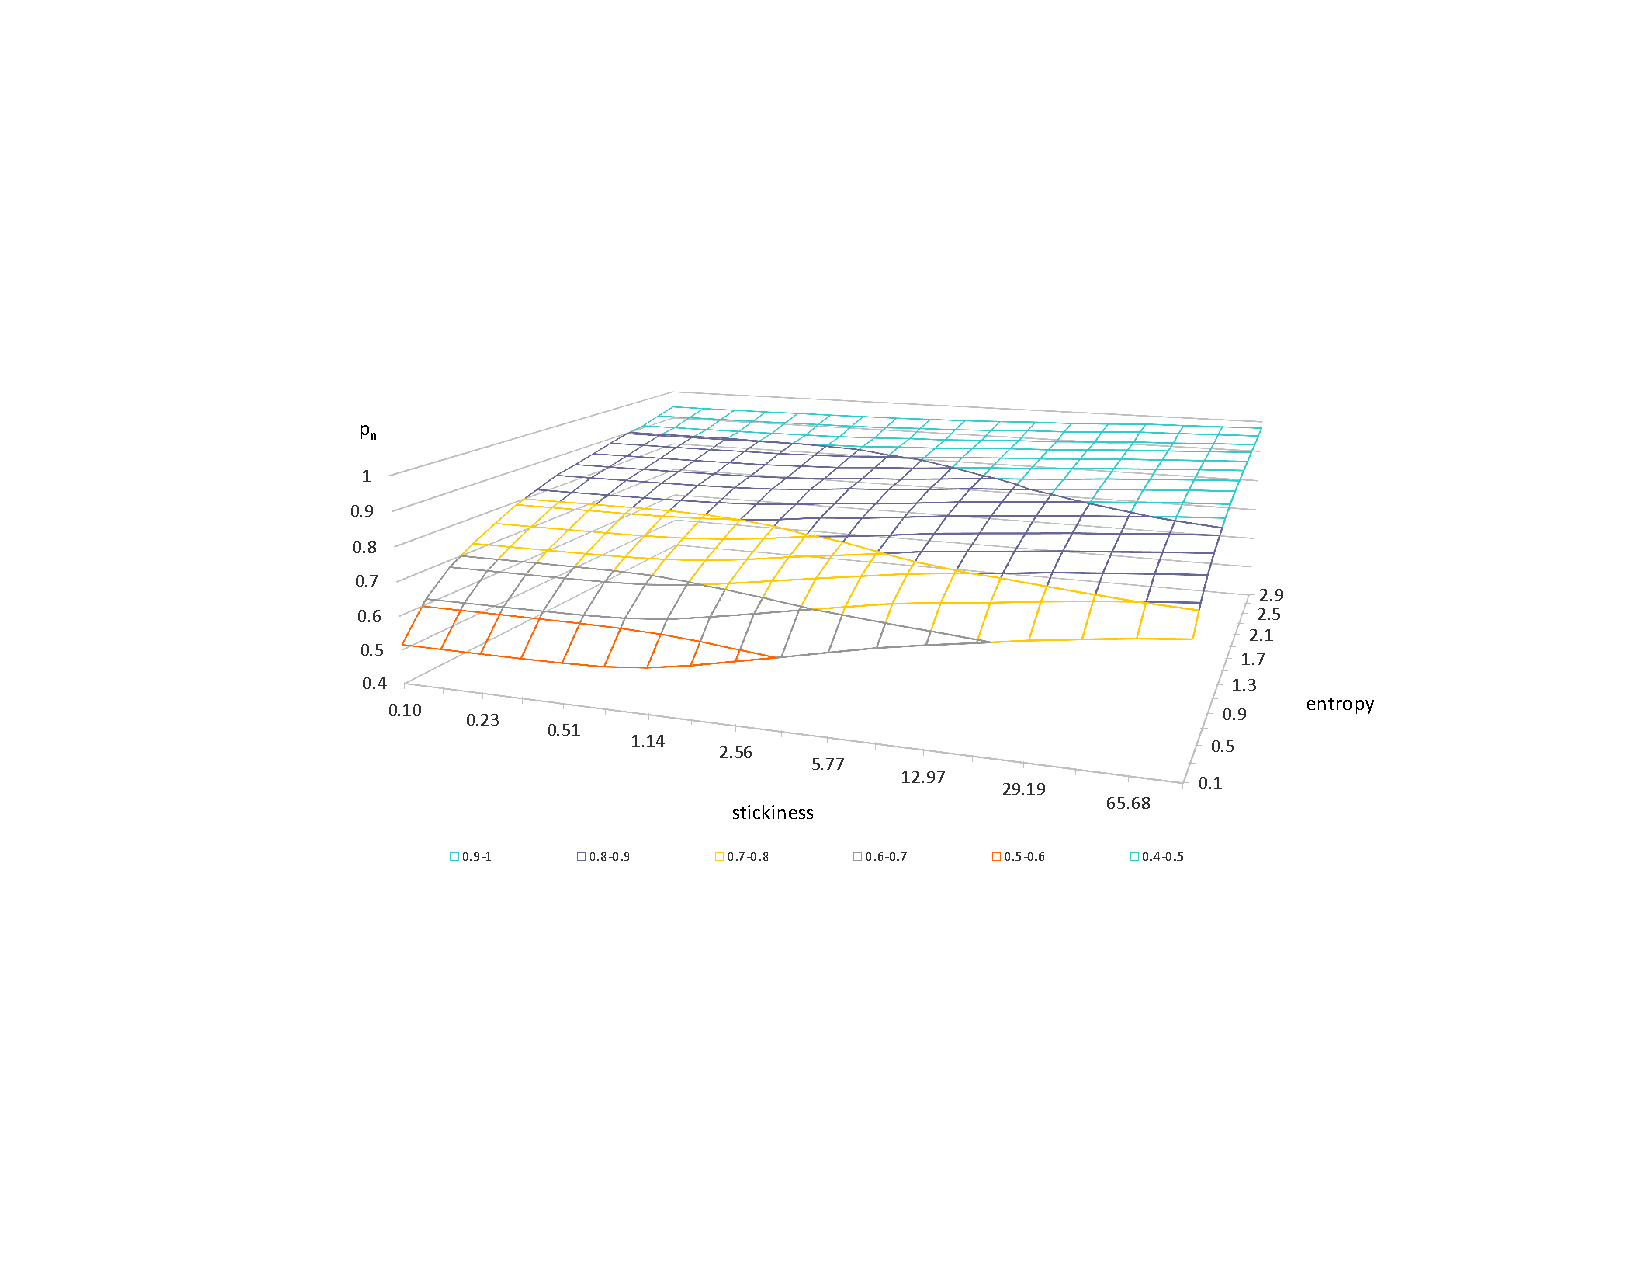
\includegraphics{figure/word_extra_pn.pdf}}
\caption{Effects of stickiness and entropy on $p_n$}
\end{figure}

$p_w$ and $p_n$ are two opposite objectives; thus, a tradeoff is required. Based on Figures \ref{weibo:fig:sepw} and \ref{weibo:fig:sepn}, stickiness $s$ and entropy $e$ are ultimately determined to be $s=5$ and $e=1$.

Moreover, the segmentation algorithm is based on the statistical property; hence, the frequency of each token is required to be $F\ge30$, to ensure that the property is statistically creditable. Another consideration when determining F is that the major intention of the algorithm is to extract financial keywords that are significant  (i.e., people extensively and frequently discuss it). Less frequently appeared words may cause the inaccuracy of the statistical model that is subsequently used in analyzing data.

\subsubsection{Keywords and Viewpoints}
Through the proposed word extraction algorithm, blog titles are separated into 1,680 tokens. These tokens undergo a manual scanning process, in which non-word tokens are deleted, obtaining a list of 1,541 words.
Among the keywords, bullish/bearish words and words that are closely related to the financial market, such as IPO and interest rate, are selected as finance-related keywords. The keyword set contains 130 words, of which 58 words are emotional and the other 72 words are neutral.

Given 130 keywords, we collect viewpoints based on the microblogs. In total, 1,098 days of data are collected (Decemeber 30, 2009 to December 31, 2012). Figure~\ref{fig:weibo:trading} shows a miniature of the viewpoints, i.e., the total number of daily posts from October 1, 2012 to December 31, 2012. The vertical axis indicates the number of daily posts summed over all of the keywords. Every bar in the chart corresponds to one day, where ``0'' and ``1'' below the bars represent non-trading and trading days, respectively. The average number of daily posts on a trading day is 862,254, more than twice as many as that on a non-trading day. This result is consistent with the common-sense idea that investors tend to discuss the stock market more on trading days. In the final analysis of this study, the data for non-trading days are removed because no corresponding index data for non-trading days exist.
\begin{figure}[htbp]
\center
\resizebox{0.5\textwidth}{!}{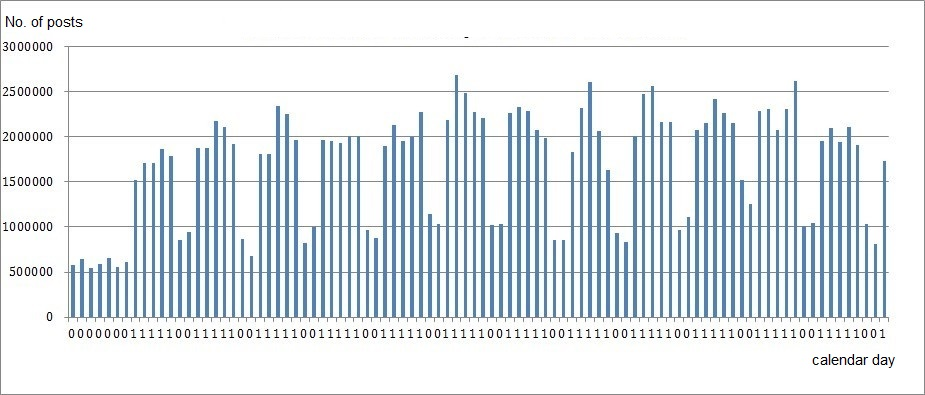
\includegraphics{figure/trading}}
\caption{Number of daily posts from October 1, 2012 to December 31, 2012}
\label{fig:weibo:trading}
\end{figure}

\subsection{Statistical Testing}
\subsubsection{Unit Root Testing}
The ADF test is applied to 130 time series $x_i$ and 1 time series $o$, so as to identify unit root processes.
The result indicates that 37 of the 130 time series of independent variables are identified as unit root processes with p-values less than 0.0001. They are denoted by I(0) and shown in Table \ref{tab:adf-test}. Dependent variable $o$ is also a unit root process. The remaining 93 time series are denoted by I(0).

\begin{table}[htbp]
\caption{Results of the ADF test}
\label{tab:adf-test}
\center
\begin{tabular} {l l}
\hline
\multirow{4}{*}{I(1)}
&  $x_1$*** $x_6$*** $x_7$*** $x_8$*** $x_{14}$*** $x_{17}$*** $x_{24}$*** $x_{31}$*** $x_{32}$*** $x_{34}$*** $x_{42}$***\\
& $x_{45}$*** $x_{47}$*** $x_{48}$*** $x_{49}$*** $x_{53}$*** $x_{55}$*** $x_{57}$*** $x_{61}$*** $x_{62}$*** $x_{77}$***\\
& $x_{78}$*** $x_{80}$*** $x_{86}$*** $x_{87}$*** $x_{91}$*** $x_{97}$*** $x_{98}$*** $x_{99}$*** $x_{100}$*** $x_{104}$***\\
& $x_{105}$*** $x_{106}$*** $x_{111}$*** $x_{115}$*** $x_{117}$*** $x_{125}$*** \\
\hline
\multicolumn{2}{l}{***p$<$0.0001}
\end{tabular}
\end{table}

The ADF test is also applied to series $r_d$; the result suggests that series $r_d$ is not a unit root process.

\subsubsection{Variable Selection}

During variable reduction, $\varepsilon_d$ is treated as white noise and the ordinary least square estimation is applied. After a stepwise variable selection procedure is deployed to the linear Model \ref{weibo:eqn:unitroot}, the total number of variables is reduced from 130 to 16. As shown in Table \ref{tab:open-variable-selection}, 11 variables are from I(0) and the other 5 variables are from I(1).

\begin{table}[htbp]
\caption{Results of the stepwise variable selection of Model \ref{weibo:eqn:unitroot}}
\label{tab:open-variable-selection}
\center
\footnotesize
\begin{tabular} {l l l p{4cm} l}
\hline
 & English meaning & mean & coefficient (Std. Error) & VIF\\
\hline
$x_2$            &moderate bullish	      &105.51	&0.121**(0.000)	    &2.781\\
$x_{10}$         &crush the market	      &38.73	&-0.276***(0.000)	&2.530\\
$x_{25}$         &real market	              &295.26	&-0.072**(0.000)	&1.257\\
$\Delta x_{32}$  &$\Delta$consolidation     &0.33	    &-0.086***(0.000)	&1.088\\
$x_{54}$         &short-term adjustment	  &15.98	&-0.166***(0.000)	&2.326\\
$x_{56}$         &bearish                   &102.63	&0.368***(0.000)	&3.557\\
$\Delta x_{61}$  &$\Delta$market adjustment &0.05	    &-0.099***(0.000)	&1.075\\
$x_{74}$         &over-sold bounce	      &70.13	&0.166***(0.000)	&4.016\\
$x_{75}$         &short squeeze	          &29.75	&0.273***(0.000)	&1.898\\
$x_{83}$         &induced buy	              &43.24	&0.085***(0.000)	&1.117\\
$\Delta x_{86}$  &$\Delta$break through      &0.15	    &0.134***(0.000)	&1.246\\
$x_{94}$         &catch rebound	          &33.45	&-0.402***(0.000)	&5.431\\
$x_{103}$        &empty position	          &172.80	&-0.303***(0.000)	&2.352\\
$\Delta x_{115}$ &$\Delta$sell high         &0.19	    &-0.079**(0.000)	&1.308\\
$\Delta x_{117}$ &$\Delta$rebound           &0.11	    &0.169***(0.000)	&1.274\\
$x_{121}$        &market rally	          &32.21	&0.199***(0.000)	&6.048\\
\hline
\multicolumn{5}{l}{Summary N = 729, Std. Error = 0.011, $R^2$ = 0.346}\\
\multicolumn{5}{l}{\quad\quad\quad\quad Adj. $R^2$ = 0.332, F = 23.571, DW = 2.328} \\
\hline
\multicolumn{5}{l}{***p$<$0.01 **p $<$ 0.05}
\end{tabular}
\end{table}

The original 130 keywords contain 58 emotional words that clearly indicate bullish/bearish views and 72 neutral finance-related words. After variable selection, 14 emotional words and 2 neutral words remain, which indicates that emotional words reflect the index price movement more heavily.

\subsubsection{Parameters of the ARIMA Model}
To decide parameter $d$ in Model \ref{eqn:error}, residuals $\hat{e}_d = r_d - \hat{r}_d$ are tested for unit root through the ADF test. The test results that are summarized in Table \ref{tab:t3} suggest that the residuals form a stationary process; therefore, setting $d = 0$ is appropriate.

\begin{table}[htbp]
\caption{Results of the ADF test on residuals}
\label{tab:t3}
\center
\begin{tabular} {l c c c}
\hline
& & $t$-statistic & Prob.\\
\hline
\multicolumn{2}{l}{ADF test statistic}	&-31.83451	&0.0000\\
test critical values	&1\% level	&-3.439105 &\\	
	&5\% level	&-2.865294	&\\
	&10\% level	&-2.568825	&\\
\hline
\end{tabular}
\end{table}


The appropriate values for $p$ and $q$ in the ARIMA model follow the framework of Box and Jenkins \cite{Box2015Time}. The autocorrelation plot in Figure \ref{fig:lag1} suggests that $\varepsilon_d$ is not white noise (i.e., at most one of $p$ and $q$ is zero). The partial autocorrelation at lag $p$ is the autocorrelation between $\hat e_d$ and $\hat e_{d-p}$. The partial autocorrelation of an AR($p$) process is zero at lag $p+1$ and greater. Similarly, the partial autocorrelation of an MA($q$) process is zero at lag $q+1$ and greater. From Figure \ref{fig:lag2}, the partial autocorrelation at lags 4, 5 and 6 is nearly zero, and setting $p$ and $q$ to be around 3 is a sensible choice.

\begin{figure}[htbp]
\centering
\subfigure[Autocorrelation for residuals $\hat{e}_d$]{
    \label{fig:lag1}
    \resizebox{0.45 \textwidth}{!}{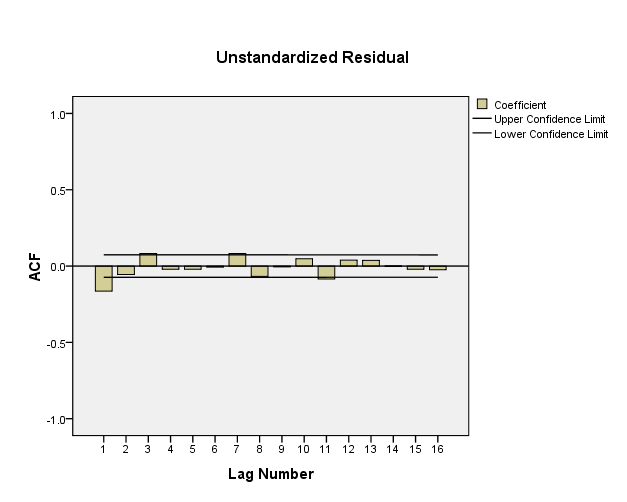
\includegraphics{figure/lag1}}}
\subfigure[Partial autocorrelation for residuals $\hat{e}_d$]{
    \label{fig:lag2}
    \resizebox{0.45 \textwidth}{!}{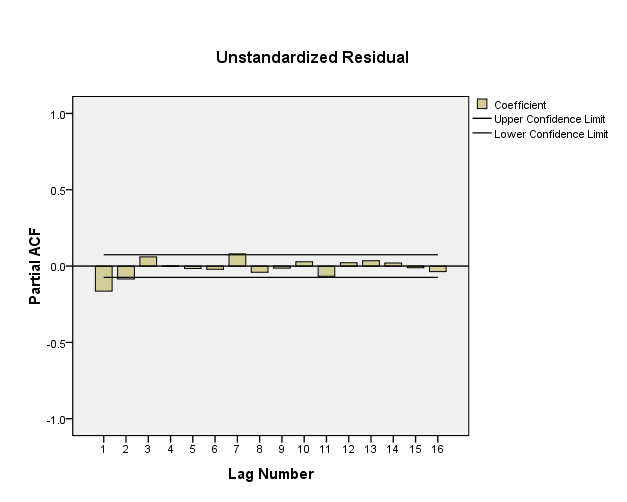
\includegraphics{figure/lag2}}}
\caption{Plot for residuals $\hat{e}_d$}
\end{figure}

Each combination of $p=0,1,2,3$ and $q=0,1,2,3$ is tested against the residuals in Model \ref{eqn:error} using the G-N iteration method. AIC, SC, and BIC are used to evaluate the fitness of models. The results are summarized in Table~\ref{tab:select-pq}.

\begin{table}[htbp]
\caption{Fitness of ARIMA$(p,0,q)$}
\center
\label{tab:select-pq}
\begin{tabular} {l c c c c}
\hline
(p,q)    & AIC & SC & N-BIC & Sig. of Ljung-Box Q (18)\\
\hline
(0,1)*** & -6,3103 & \bf{-6.3040} & \bf{-9.140} & 0.236 \\
(0,2)	 &-6.3085	&-6.2959	&-9.131	&0.235\\
(0,3)	 &-6.3111	&-6.2922	&-9.126	&0.459\\
(1,0)***	&-6.3062	&-6.2999	&-9.137	&0.099\\
(1,1)	 &-6.3072	&-6.2946	&-9.131	&0.211\\
(1,2)***	&-6.3103	&-6.2914	&-9.121	&0.128\\
(1,3)	 &-6.3090	&-6.2838	&-9.117	&0.462\\
(2,0)**	 &-6.3102	&-6.2976	&-9.134	&0.397\\
(2,1)	 &-6.3104	&-6.2914	&-9.126	&0.503\\
(2,2)	 &-6.3092	&-6.2839	&-9.118	&0.457\\
(2,3)***	&-6.3180	&-6.2865	&-9.110	&0.475\\
(3,0)	 &-6.3101	&-6.2912	&-9.127	&0.525\\
(3,1)	 &-6.3075	&-6.2822	&-9.116	&0.449\\
(3,2)**	 &\bf{-6.3214}	&-6.2898	&-9.110	&\bf{0.503}\\
(3,3)	 &-6.3186	&-6.2807	&-9.100	&0.284\\
\hline
\multicolumn{5}{l}{***p$<$0.01 **p $<$ 0.05}
\end{tabular}
\end{table}

Parameter combinations that induce the best fitness in terms of one selection criterion are highlighted in bold. According to the AIC criterion, ARIMA(3,0,2) is the best model. According to SC and BIC criteria, ARIMA(0,0,1) is the best model.

ARIMA(0,0,1) and ARIMA(3,0,2) are subsequently tested against the merged model. If the error term $\varepsilon_d$ can be adequately modeled by ARIMA(0,0,1), then the complete model is simplified as follows:
\begin{equation}
    \ln \frac{o_d}{o_{d-1}} = \alpha_0 + \sum_{x_i \in J(0)} \alpha_i x_{i,d-1} + \sum_{x_i \in J(1)} \alpha_i \Delta x_{i,d-1} + (1 + \theta_1 L) \eta_d \label{eqn:arima1}
\end{equation}
where J(0)=\{ $x_2$, $x_{10}$, $x_{25}$, $x_{54}$, $x_{56}$, $x_{74}$, $x_{75}$, $x_{83}$, $x_{94}$, $x_{103}$, $x_{121}$\} and J(1) = \{$x_{32}$, $x_{61}$, $x_{86}$, $x_{115}$, $x_{117}$\}.

If the error term $\varepsilon_d$ can be adequately modeled by ARIMA(3,0,2), the complete model is simplified as follows:
\begin{eqnarray}
    \ln \frac{o_d}{o_{d-1}} & = & \alpha_0 + \sum_{x_i \in J(0)} \alpha_i x_{i,d-1} + \sum_{x_i \in J(1)} \alpha_i \Delta x_{i,d-1} \nonumber \\
                           & + & (1-\phi_1L-\phi_2L^2-\phi_3L^3)^{-1}(1 + \theta_1 L + \theta_2 L^2) \eta_d \label{eqn:arima32}
\end{eqnarray}

The parameters in the preceding two models are estimated using the G-N iteration method and the comparative results are summarized in Table \ref{tab:comp}. Model \ref{eqn:arima32} achieves a higher stationary $R^2$, and is a better model.

\begin{table}[htbp]
\caption{Comparison of Models \ref{eqn:arima1} and \ref{eqn:arima32}}
\label{tab:comp}
\center
\begin{tabular} {l c c c c c}
\hline
Model                   & stationary $R^2$ & SER   & DW    & AIC   & Sig. of L-B Q (18)\\
\hline
Model \ref{eqn:arima1}  & 0.367            & 0.804 & 1.989 & 2.422 & 0.244\\
Model \ref{eqn:arima32} & 0.374            & 0.797 & 2.00  & 2.412 & 0.468\\
\hline
\end{tabular}
\end{table}

The estimated parameters for Model \ref{eqn:arima32} are presented in Table \ref{tab:arima32-open}. Results suggest a correlation between the daily opening price and the number of related posts on Sina Weibo. Positive terms such as ``moderate bullish," ``over-sold rebound," and ``short squeeze" are positively correlated with the daily opening price; by contrast negative terms such as ``crush the market" and ``empty position" are negatively correlated with the stock index. However, a few exceptions exist. For example, the term ``bearish" expresses a negative view on the stock market, but it has a positive effect on the stock index in the proposed model.

\begin{table}[htbp]
\caption{Estimated parameters of Model \ref{eqn:arima32}}
\scriptsize
\center
\label{tab:arima32-open}
\begin{tabular} {l l p{2.3cm}|| l l p{2.3cm}}
\hline
variable         &	English meaning	     & coefficient (Std. Error)&	variable      &	English meaning      &	coefficient (Std. Error)\\
\hline
$x_2$            & moderate bullish	     &0.085***(0.033)          & $x_{94}$         &catch rebound         & -0.307***(0.048) \\
\hline
$x_{10}$         & crush the market	     &-0.172***(0.032)         & $x_{103}$        &empty position	     & -0.246***(0.035) \\
\hline
$x_{25}$         &real market	         &-0.054*(0.029)           & $\Delta x_{115}$        & $\Delta$ sell high	     & -0.138***(0.037) \\
\hline
$\Delta x_{32}$  & $\Delta$consolidation &-0.107***(0.033)         & $\Delta x_{117}$ & $\Delta$rebound      & 0.150***(0.032) \\
\hline
$x_{54}$         &short-term adjustment	 &-0.105***(0.031)         & $x_{121}$        &market rally	         & 0.112**(0.045) \\
\hline
$x_{56}$         &bearish	             &0.289***(0.044)	       &$\phi_1$	      &---	                 & -0.791***(0.178)\\
\hline
$\Delta x_{61}$  &$\Delta$market adjustment  &-0.104***(0.032)	   &$\phi_2$	      &---	                 & -0.829***(0.136)\\
\hline
$x_{74}$         &over-sold bounce	     &0.143***(0.045)	       &$\phi_3$	      &---	                 & -0.134**(0.055)\\
\hline
$x_{75}$         &short squeeze	         &0.225***(0.030)	       &$\theta_1$	      &---	                 & 0.591***(0.175)\\
\hline
$x_{83}$         &induced buy	         &0.086***(0.029)	       &$\theta_2$	      &---	                 & 0.685***(0.128)\\
\hline
$\Delta x_{86}$  & $\Delta$break through & 0.160***(0.034)\\

\hline
\multicolumn{6}{l}{***p$<$0.01  **p$<$0.05  *p$<$0.1}
\end{tabular}
\end{table}

\subsubsection{Model Validation}

The validity of the model is tested by standard procedures. First, the moduli of the inverse of the AR roots are 0.872, 0.872, and 0.176, and the moduli of the inverse of the MA roots are 0.827 and 0.827. The inverses of all of the roots lie inside the unit circle in Figure \ref{fig:inverroot}; therefore, 3 is not a unit root in the fitted ARIMA(3,0,2) model. A first-order autoregressive conditional heteroskedasticity test on the residuals suggests no obvious heteroscedasticity. $DW=2$ indicates the lack of strong autocorrelation. The autocorrelation coefficients of the residuals are very close to zero [refer to Figure \ref{fig:ACF}]. The Ljung-Box $Q$ value is equal to 0.495\footnote{This weak hypothesis test infers that the residuals are white noise. The null hypothesis is that the residuals are not white noise.}, which suggests that the residuals are likely to be white noise. In summary, the model is valid.

\begin{figure*}[htbp]
\centering
\subfigure[Inverses of AR and MA roots]{
    \label{fig:inverroot}
    \resizebox{0.35 \textwidth}{!}{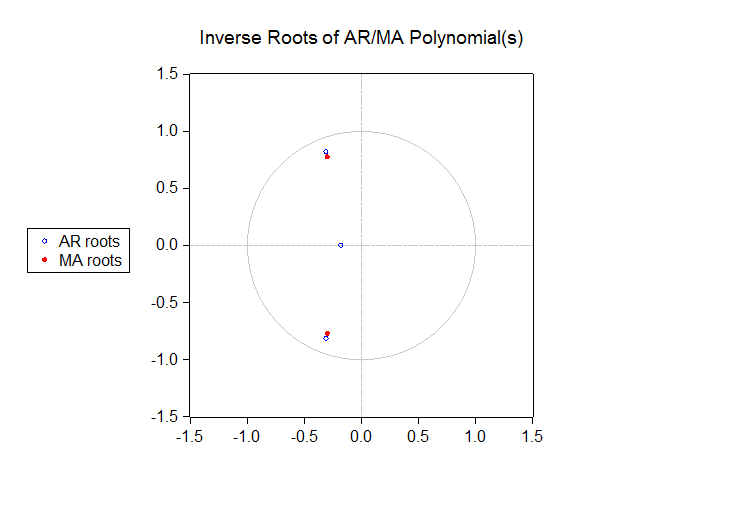
\includegraphics{figure/inverse_root_of_ARIMA}}}
\subfigure[ACF and PACF of residuals]{
    \label{fig:ACF}
    \resizebox{0.45 \textwidth}{!}{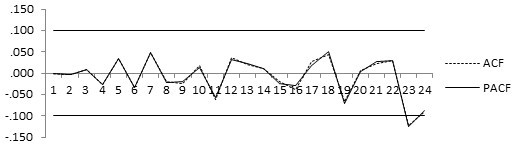
\includegraphics{figure/ACF}}}
\caption{Model validity}
\end{figure*}

Based on the fitted model, actual daily open prices, fitted values, and residuals are plotted in Figure \ref{fig:result}. The horizontal axis represents the time in days. The residuals in the early days are slightly larger. As time passes, the fitness becomes better as the residuals become smaller and more stable.
\begin{figure*}[htbp]
\center
\resizebox{0.45 \textwidth}{!}{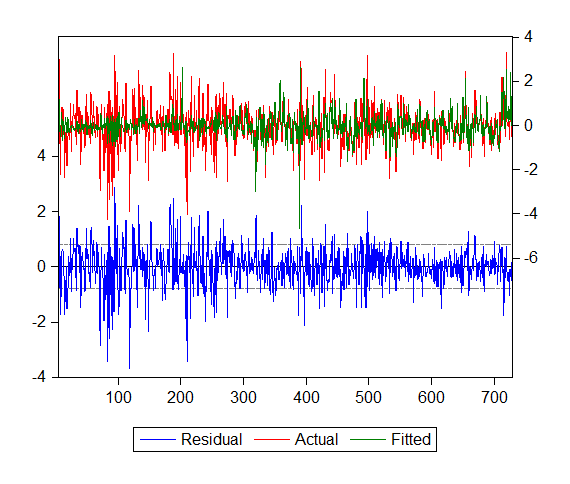
\includegraphics{figure/regression_result}}
\caption{Actual and fitted values of daily opening prices}
\label{fig:result}
\end{figure*}

The causality between market returns and keywords of Weibo posts is tested by a Granger causality test. The results are shown in Table \ref{tab:weibo:grangerCausality}. With a 5\% significant level, the price movement does not Granger-cause the posts, except five words (i.e., short-term adjustment, market adjustment, over-sold bounce, rebound, and market rally). Moreover, all of the posts of the keywords, except real market and consolidation, Granger-cause the price movement. Thus, posts affect the market, but the market does not affect the posts.

\begin{table}[htbp]
\caption{ Results of the Granger causality test}
\footnotesize
\center
\label{tab:weibo:grangerCausality}
\begin{tabular}{r p{3cm} r|| p{3cm} r}
\hline
        $x_i$ & F-statistic (price movement does not Granger-causes $x_i$) &      Prob. & F-Satistic ($x_i$ does not Granger-causes price movement) &      Prob. \\
\hline
moderate bullish      &      1.011 &     0.3656 &     42.415 &   2.00E-16 \\

crush the market      &      1.845 &     0.1603 &     43.479 &   9.00E-17 \\

real market           &      2.539 &     0.0811 &    0.00408 &     0.9959 \\

consolidation         &      2.169 &     0.1165 &      2.531 &     0.0817 \\

short-term adjustment &      15.83 &   4.00E-07 &      5.372 &     0.0052 \\

   bearish            &      0.537 &     0.5853 &     23.191 &   6.00E-10 \\

market adjustment     &      14.95 &   8.00E-07 &      15.95 &   3.00E-07 \\

over-sold bounce      &     11.792 &   1.00E-05 &      9.439 &     0.0001 \\

short squeeze         &      0.502 &     0.6061 &     35.763 &   3.00E-14 \\

induced buy           &      0.097 &     0.9069 &      8.661 &     0.0002 \\

break through          &      0.314 &     0.7305 &     20.731 &   5.00E-09 \\

catch rebound         &      0.076 &     0.9266 &      26.55 &   4.00E-11 \\

empty position        &      0.131 &     0.8774 &      13.84 &   2.00E-06 \\

 sell high            &      2.157 &     0.1179 &      6.771 &     0.0014 \\

   rebound            &        4.7 &     0.0001 &     12.801 &   5.00E-06 \\

market rally &     7.6577 &     0.0006 &     23.145 &   7.00E-10 \\
\hline
\end{tabular}
\end{table}

\subsection{Discussion}
\label{sect:result}
\vspace{5mm}
Sina Weibo is the largest microblog in China. What is more, according to the annual report of Weibo user development 2017, the users are highly educated, and most of the users are students in universities and white collar. Hence, the topics discussed in the microblog are mostly about politics, policy, economy, stock market, culture, and entertainment. The viewpoints in Weibo are typical and reliable.\\
\indent
The short-term performance of a stock is often driven by the arrival of new information, such as the announcements of profit warnings, major asset acquisitions, and new policies. In terms of stock prices, delays between the time of announcements and stock price response occur. Stock prices usually respond in a matter of hours or even days because information requires time to propagate through the major media until it reaches the majority of the population. An announcement is initially reported in less popular media or the website of the company. As the exposure increases, a sufficiently large proportion of the population becomes interested. The news becomes a hot topic and appears as headlines in many major media, which in turn quickly increases the exposure. After a piece of news reaches an investor, the investor requires time to digest and understand its implications. Depending on the complexity of the matter, the majority of investors may require minutes, hours, days, or even months (considering a major policy change) to digest the information.\\
\indent
In the information propagation and digestion process, some individual investors will share their viewpoints via Sina Weibo due to the sheer number of active users and the real-time feature of Sina Weibo. With the development of computer programs to source the continuous flows of news from the Internet and to automatically analyze sentiments, the viewpoints of a large group of individual investors can indeed be captured in a timely manner. If the lag of stock price response to news occurs and the aggregated viewpoints of individual investors can be accessed before a new price forms, then people can predict the price movement, take advantage of the posts, and modify the prediction as more posts are explored. Thus, predicting price trends is possible based on the correlation between the viewpoints of individual investors and stock market movements.


\section{Conclusions}
\label{sec:weibo:conclude}
The proliferation of the Internet has improved our ability to access information in real time. The Internet has evolved substantially over the last 30 years, and it has become a source of information of nearly every aspect of our lives. Social media is a particular implementation that has grown considerably in the 21st century.

Social media is a valuable source for polling public views. The rapid development of social media and technology in text mining not only allows us to collect opinions from a large group of individuals, but also to perform this task in a timely manner.

Automatic word segmentation algorithm is illustrated in this study. Conventionally, empirical researchers select keywords manually, and this approach is subjective to some extent. The proposed method can avoid the bias of personal experience and is more robust and objective. The collected posts are used to measure the collective viewpoints of individual investors, particularly their emotions. The ARIMA model is deployed to link the collective viewpoints and the movements of the Chinese stock market, and a Granger test is performed to verify the causality relationship between the two variables. The statistical results infer that viewpoints reveal market movements.

Social media can be transformed into a powerful source of data using the appropriate text mining tools. Given that the short-term stock market is affected by financial news, information propagation and digestion require time. The findings in this paper provide evidence for predicting market movements based on the promptly collected online viewpoints (emotions) of investors.


%\section*{Acknowledgments}
%
%This research was partially supported by the National Natural Science Foundation of China (No.\ 71602109), Shanghai Pujiang Program (No.\ 16PJC038), and Funding Program for Teachers of Shanghai High Education (No.\ ZZSD15095).



\bibliographystyle{ieeetr}%apalike2
\bibliography{weibo}
\end{document}











